\begin{section}{Conceptos}
En este apartado se describen algunos conceptos que se deben tener claros para entender la estructura y arquitectura de los componentes de VMware Cloud Foundation.
% En este apartado se describe la arquitectura de VMware Cloud Foundation y como estructura sus componentes\footnote{Se describen solo aquellos componentes que se utilizarán en el despliegue de Cloud Foundation.} internamente.

%%%%%%%%%%%%%%%%%%%%%%%%%%%%%%
% \iffalse
% En este apartado se explican aquellos conceptos de VMware Cloud Foundation necesarios para entender su funcionamiento, configuración y requisitos de la infraestructura previos al despliegue del servicio.
% \fi
%%%%%%%%%%%%%%%%%%%%%%%%%%%%%%%%


%% Workload Ddomains %&%&%%%%
%%%%%%%%%%%%%%%%%%%%%%%%%%%%
\begin{subsection}{Workload Domain}
Un \textit{workload domain} (WD) representa un bloque de recursos dentro del SDDC, que son componentes de la infraestructura física, de la infraestructura virtual, y de seguridad. Los componentes virtuales controlan el acceso y la reserva de los recursos físicos, mientras que la capa de seguridad permite establecer organizar la entrada al WD. Cada WD contiene sus propias instancias de VMware ESXi, VMware vCenter Server, VMware NSX-T y VMware vSAN, pudiendo así gestionar los recursos de cada WD de forma independiente.
% Un \textit{workload domain} consiste en una instancia lógica de un SDDC que abarca todos o parte de los recursos de uno o más clusters, cuya función es aislar el flujo de trabajo de un usuario, aplicación o un determinado tipo de tareas. Cada \textit{workload domain} se extiende sobre varios hosts con el hipervisor ESXi, y contiene sus propias instancias de VMware vCenter Server, VMware vSAN y VMware NSX-T. Así, esta arquitectura permite establecer políticas de control específicas para un \textit{workload domain} y otras comunes para todos o varios \textit{workload domains} y específicas para cada uno de ellos a la vez que se simplifica la complejidad de la infraestructura. Existen \underline{tres tipos} de \textit{workload domains} que permiten aislar las tareas de gestión de la infraestructura del resto de flujos de trabajo. 

%% MANAGEMENT DOMAIN
\begin{subsubsection}{Management Domain}
\label{subsubsec:domainManagement}
% Este \textit{workload domain} se crea y configura automáticamente durante el proceso de despliegue de una instancia de VMware Cloud Foundation.
El \textit{management domain} es el primer WD que se crea dentro del SDDC, y su función es la gestión de todos los componentes de VMware Cloud Foundation, tanto del propio \textit{management domain} como del resto de \textit{workload domains} existentes.
En este \textit{workload domain} se genera un cluster de VMware vSphere donde se despliegan las instancias de los siguientes componentes:
\begin{itemize}
  \item Una VM de SDDC Manager.
  \item Una VM de VMware vCenter Server.
  \item Tres VMs de VMware NSX-T Manager Appliance.
  \item Dos VMs de VMware NSX-T Edge.
\end{itemize}
El administrador gestiona los recursos del \textit{management domain} desde VMware vSphere Client, VMware NSX-T Manager (para gestionar sus redes virtuales) y VMware SDDC Manager para administrar los aspectos que afectan a todo el SDDC como puede ser la instalación de otras aplicaciones de VMware o la creación de nuevos \textit{workload domains}. 
% Incluye las siguientes instancias: SDDC Manager, vCenter Server, una instancia de NSX Manager, tres instancias de NSX Controller, dos instancias de Platform Services Controller y tres instancias de vRealize Log Insight \cite{sddcComponents} [Fig. \ref{fig:componentsMNGDomain}].\\
% Cuando se \underline{despliega \textit{management domain} se crean y configuran} de forma automatizada por SDDC Manager las siguientes máquinas virtuales (VM) de cada componente de Cloud Foundation\footnote{Las características de cada máquina virtual se refieren a los requisitos mínimos}:
% \begin{itemize}
%     \item Una VM de \textbf{SDDC Manager}: 4 vCPU, 16 GB de memoria, 800 GB de almacenamiento.
%     \item Una VM de \textbf{vCenter Server}: 4 vCPU, 16 GB de memoria, 290 GB de almacenamiento.
%     \item Dos instancias de \textbf{Platform Services Controller} (cada una): 2 vCPU, 4 GB de memoria, 60 GB de almacenamiento.
%     \item Una VM de \textbf{NSX Manager}: 4 vCPU, 16 GB de memoria, 60 GB de almacenamiento.
%     \item Tres VM de \textbf{NSX Controller} (cada una): 4 vCPU, 4 GB de memoria, 28 GB de almacenamiento.
%     \item Tres VM de \textbf{vRealize Log Insight}: 4 vCPU, 8 GB de memoria, 250 GB de almacenamiento.
% \end{itemize}

% Para desplegar el \textit{management domain} se requieren las siguientes \underline{capacidades mínimas} en la infraestructura \cite{WDminRequierements}:
% \begin{itemize}
%     \item \textbf{Hosts}: 4
%     \item \textbf{CPU} por host: Dual-socket con 8 cores por socket, en sistemas All-Flash.
%     \item \textbf{Memoria} total: 192 GB
%     \item \textbf{Almacenamiento} por host: 16 GB para el dispositivo de arranque, un NVMe o SSD para la capa de caché, dos SSD o HDD para la capa de capacidad\footnote{En total se requieren 800 GB para este \textit{workload domain}.}.
%     \item \textbf{NICs} por host: Dos NICs de al menos 10 GbE y, opcionalmente un NIC 1GbE BMC.
% \end{itemize}

% \begin{figure}[h!]
%   \centering
%   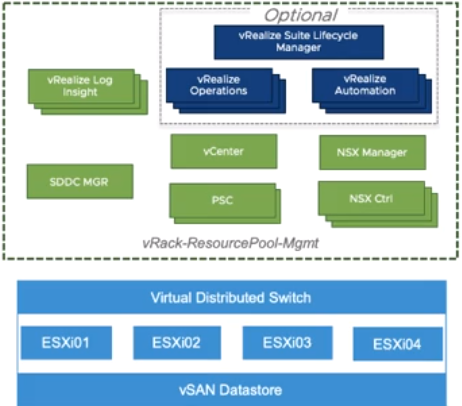
\includegraphics[width=0.5\textwidth]{imaxes/conceptosPrevios/componentsMANAGEDomain.png}
%   \caption{Componentes de \textit{management domain}}
%   \label{fig:componentsMNGDomain}
% \end{figure}
\end{subsubsection}

%% VIRTUAL INF. DOMAIN
\begin{subsubsection}{Virtual Infrastructure Domain (VI)}
\label{subsubsec:domainVI}
Este tipo de \textit{workload domain} se crea manualmente y bajo demanda desde \textit{management domain} para habilitar entornos con una finalidad diferente. Su configuración de hardware y lógica se especifican durante su proceso de creación, permitiendo indicar la cantidad de hosts, cantidad de almacenamiento, configuración de la red y políticas de rendimiento y disponibilidad, todo para satisfacer las necesidades del tipo de tareas para las que se crea. Con cada \textit{workload domain} se genera un nuevo cluster de VMware vSphere que agrupa los nuevos recursos pero parte de sus componentes que se despliegan se controlan desde el \textit{management domain}:
\begin{itemize}
  \item Una VM de VMware vCenter Server.
  \item Tres VMs de VMware NSX-T Manager Appliance situadas en el \textit{management domain}.
  \item Dos VMs de VMware NSX-T Edge.
\end{itemize}
El administrador gestiona los recursos del \textit{VI domain} desde VMware vSphere Client y la instancia de SDDC Manager situada en el \textit{management domain}, y gestiona las redes virtuales del \textit{workload domain} desde VMware NSX-T Manager situado también en el \textit{management domain}.
% La diferencia entre un \textit{virtual infrastructure domain} y \textit{virtual desktop infrastructure domain} es que el segundo incorpora el producto VMware Horizon View que, resumiendo, permite desplegar escritorios virtuales. 
% Con cada nuevo \textit{virtual infrastructure domain} se crea un nuevo cluster vSphere en la infraestructura que agrupa todos los recursos que tiene asignados.\\
% Cuando se \underline{despliega un \textit{virtual infrastructure domain} se crean y configuran} de forma automatizada por el componente SDDC Manager las siguientes máquinas virtuales (VM) de cada componente de VMware Cloud Foundation\footnote{Las características de cada máquina virtual se refieren a los requisitos mínimos} 
%\cite{sddcComponents} [Fig. \ref{fig:compoVIdomain}]:
% \begin{itemize}
%     \item Una VM de \textbf{vCenter Server} en Management Domain: 8 vCPU, 24 GB de memoria, 500 GB de almacenamiento.
%     \item Una VM de \textbf{NSX Manager} en Management Domain: 4 vCPU, 16 GB de memoria, 60 GB de almacenamiento.
%     \item Tres VM de \textbf{NSX Controller} en el VI Domain creado (cada una):  4 vCPU, 4 GB de memoria, 28 GB de almacenamiento.
% \end{itemize}

% Por cada \textit{virtual infraestructure domain} que se despliega en la infraestructura, se requieren las siguientes capacidades mínimas\cite{WDminRequierements}:
% \begin{itemize}
%     \item \textbf{Hosts}: 3
%     \item \textbf{CPU}, \textbf{Memoria} y \textbf{Almacenamiento}: depende de los requisitos de las tareas que se vayan a desarrollar en este \textit{workload domain}.
%     \item \textbf{NICs} por servidor: Dos NICs de al menos 10 GbE y, opcionalmente un NIC 1 GbE BMC.
% \end{itemize}


 \end{subsubsection}

\end{subsection}
% \begin{figure}[h!]
%   \centering
%   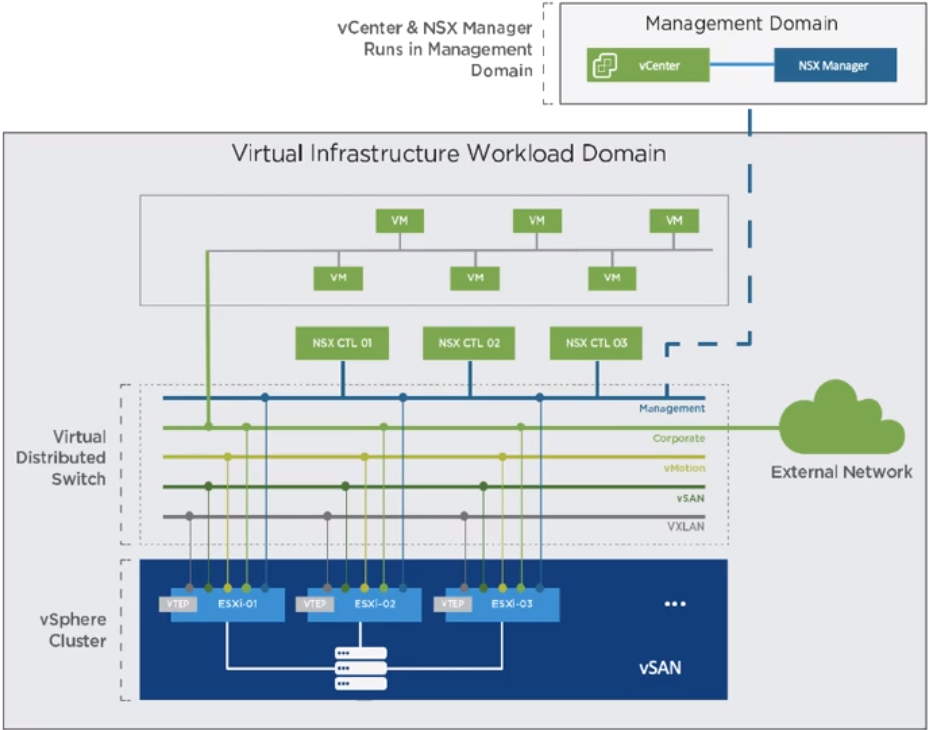
\includegraphics[width=0.5\textwidth]{imaxes/conceptosPrevios/networkArcVIDomain.png}
%   \caption{Componentes de \textit{virtual infrastructure domain}.}
%   \label{fig:compoVIdomain}
% \end{figure}
%\FloatBarrier

%&%%%%%%%%%%%%%%%%%%%%%%%%%%%%%%%%%%%%%%%%%%%%%%%%%%%%%%%%
%% ARQUITECTURA



\begin{subsection}{Arquitectura}
La arquitectura de VMware Cloud Foundation tiene dos posibles modelos de despliegue dependiendo del número de hosts sobre los que se despliega VMware Cloud Foundation.
%%%%%%%%%%%%%%%%%%%%%%%%
%%%%%%%%%%%%%%%%%%%%%%%%
%% ESTANDAR
\begin{subsubsection}{Modelo estándar}
Este modelo está pensado para desplegar VMware Cloud Foundation en entornos de tamaño medio/grande con un mínimo de siete hosts. Está formado por un \textit{management domain} que se despliega en cuatro de los hosts y contiene todos los componentes de gestión de toda la infraestructura, desde este \textit{workload domain} se administra la infraestructura del SDDC y cada \textit{virtual infrastructure domain} existente. Además, este modelo contiene al menos un \textit{virtual infrastructure domain}, creado bajo demanda y con capacidades establecidas según su finalidad que posteriormente se pueden pueden modificar, se despliega sobre al menos tres hosts. Un \textit{management domain} puede gestionar un máximo de de catorce \textit{virtual infrastructure domains}.
%Cada \textit{virtual infrastructure domain} requiere tres hosts adicionales, es decir, un host solo puede pertenecer a un único \textit{workload domain}. 

\begin{figure}[h!]
  \centering
  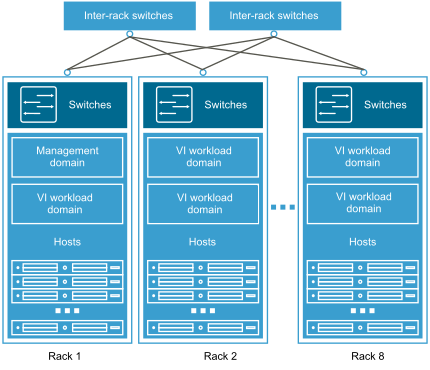
\includegraphics[width=0.6\textwidth]{imaxes/conceptosPrevios/arquitect_standarCF.png}
  \caption{Esquema del modelo de arquitectura estándar.}
  \label{fig:modelostandard}
\end{figure}

\begin{figure}[h!]
  \centering
  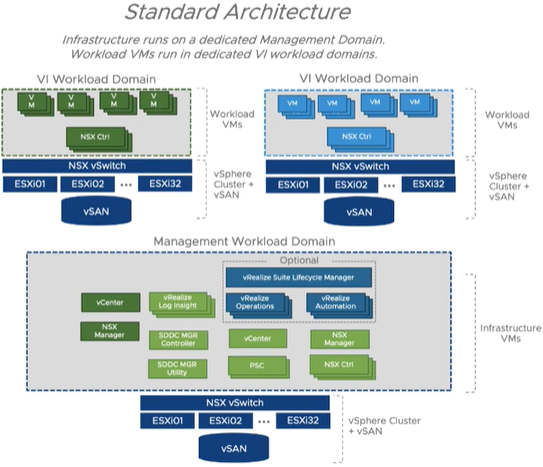
\includegraphics[width=0.6\textwidth]{imaxes/conceptosPrevios/standardArch.png}
  \caption{Estructura de los componentes en una arquitectura estándar.}
  \label{fig:standardarch}
\end{figure}
\FloatBarrier
%%%%%%%%%%%%%%%%%%%%%
%%  CONSOLIDADO
\end{subsubsection}
\begin{subsubsection}{Modelo consolidado}
Este modelo está pensado para desplegar VMware Cloud Foundation en entornos de tamaño pequeño, normalmente cuando hay menos de siete hosts, aunque se puede también se puede utilizar sobre entornos más grandes de hasta 64 hosts. En este modelo los flujos de trabajo que corresponden al \textit{virtual infrastructure domain} y al \textit{management domain} en el despliegue estándar, están colocados dentro de un mismo \textit{workload domain} en un único cluster pero aislados gracias a que cada uno se coloca dentro de un \textit{resource pool} diferente, es decir, existe un cluster con varios \textit{resource pool}. El modelo consolidado se convierte en un modelo estándar cuando se añade un \textit{workload domain} al SDDC.[Fig. \ref{fig:modeloconsolidated}].

\begin{figure}[h!]
  \centering
  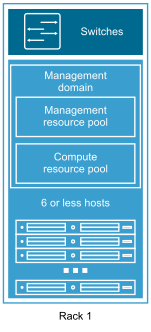
\includegraphics[width=0.25\textwidth]{imaxes/conceptosPrevios/modelConsolidated.png}
  \caption{Esquema del modelo de arquitectura consolidado.}
  \label{fig:modeloconsolidated}
\end{figure}

\begin{figure}[h!]
  \centering
  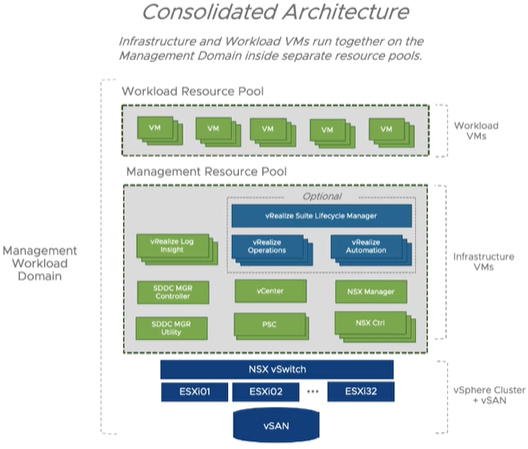
\includegraphics[width=0.6\textwidth]{imaxes/conceptosPrevios/consolidatedArch.png}
  \caption{Estructura de los componentes de una arquitectura consolidado.}
  \label{fig:consolidatedArch}
\end{figure}
\FloatBarrier

\end{subsubsection}
\end{subsection}

\begin{subsection}{Clusters, zonas y distribución de un SDDC}
\begin{subsubsection}{AZ y Region}
Los recursos de un SDDC pueden estar distribuídos en diferentes localizaciones para proporcionar alta disponibilidad y posibilidad de recuperación ante fallos. Los recursos de una o varias ubicaciones se agrupan para formar una estructura que permite usar y gestionar los recursos disponibles de forma conjunta y dinámica. Los componentes de esta estructura son:
\begin{itemize}
  \item Availability Zone (AZ): conjunto de recursos físicos que forman una infraestructura independiente para evitar la propagación de fallos hacia otras AZs. Cuando existen varias AZ estas se pueden usar de forma que cuando ocurre un fallo en una de ellas la carga de trabajo se mueve a una segunda AZ para minimizar el tiempo de caída del servicio.
  
  \item Region: conjunto de AZs gestionadas que representa una instancia del SDDC. Las AZs que la forman deben tener una latencia de 5 ms como máximo mientras que la latencia entre Regions debe ser de al menos 100 ms. Esta estructura permite acercar el servicio a ubicaciones separadas por grandes distancias. La arquitectura del modelo consolidado solo soporta una Region con una AZ, mientras que el modelo estandar permite desplegar múltiples Regions con múltiples AZs.
\end{itemize} 
\end{subsubsection}
\begin{subsubsection}{Cluster y Resource Pool}
Dentro de un \textit{workload domain} pueden existir varios clusters. Un cluster es una agrupación de hosts a cuyos recursos se les puede aplicar una una configuración deternminada con los componentes VMware vSphere High Availability y VMware vSphere Distributed Resource Scheduler para reestablecer el servicio en caso de fallos en alguno de los hosts. Un cluster puede estar extendido en más de una AZ para que si una de las AZs falla, las aplicaciones que corrían en ella pueden ser migradas a otra AZ. En un WD se despliegan dos clusters:
\begin{itemize}
  \item Management cluster: es el cluster que se crea al desplegar VMware Cloud Foundation. Contiene los componentes para administrar los recursos del WD.
  \item Shared Edge and Workload Cluster: después del management cluster, este es el primero que se crea. Su finalidad es alojar las aplicaciones y cargas de trabajo de los usuarios dentro de un WD. Además contiene instancias de Vmware NSX-T para proporcionar sevicios de red.
\end{itemize}

Dentro de un cluster se pueden crear resource pools. Un \textit{resource pool} es una carcaterística de VMware vSphere que permite abstraer un conjunto de recursos de un cluster estableciendo unos límites de capacidad que puede usar \cite{resourcePool}. Usar resource pools permite agrupar las VMs con una finalidad similar y controlar la cantidad de recursos del WD que esas VMs pueden consumir.

% Un SDDC puede estar distribuído en una o más \textit{Availability Zone} (AZ). Estas son zonas aisladas con infraestructuras independientes que evitan la propagación de fallos de hosts individuales a través de toda la infraestructura, cuantas más \textit{AZ} existan mayor disponibilidad tendrá el servicio. La latencia entre dos \textit{AZ} debe ser de 5 ms como máximo y la conexión de al menos 10 Gbit. Una \textit{Region} agrupa una o más \textit{AZ}s, con esto se da solución a la recuperación del servicio ante desastres. La latencia entre dos \textit{Region}s debe ser de 100 ms como máximo. El \underline{modelo consolidado} solo da soporte a una \textit{Region} con una \textit{AZ}, mientras que el \underline{modelo estándar} puede soportar múltiples \textit{Region} con múltiples \textit{AZ}.
\end{subsubsection}
\end{subsection}

\end{section}

% \subsubsection{Clusters, zonas de disponibilidad y regiones}
% Un SDDC puede estar formado por uno o más clusters de distintos tipos. En el  \underline{modelo consolidado} la infraestructura está formada por un único cluster que incluye los servicios de gestión de VMware Cloud Foundation VMware vCenter Server, vSphere Update Manager, VMware NSX Manager, VMware NSX Controller y VMware vRealize Log Insight, los servicios de red necesarios para establecer conectividad en el entorno y las máquinas virtuales que los usuarios crean cuando aprovisionan sus recursos. Se aplican las mismas políticas de alta disponibilidad y gestión del ciclo de vida al flujo de trabajo de gestión del SDDC y al flujo de trabajo del usuario. En el \underline{modelo estándar} los distintos \textit{workload domain} se dividen en clusters que pueden ser de tres tipos:
%     \begin{itemize}
%         \item \textbf{Management Cluster}: se crea durante el despliegue de VMware Cloud Foundation y contiene el \textit{management domain}, desde aquí se gestiona el SDDC. Contiene los servicios de gestión mecionados anteriormente.
%         \item \textbf{Shared Edge and Compute Cluster}: es el primer cluster que se crea dentro de un \textit{virtual infrastructure domain} ya que puede haber más de un cluster. Este cluster contiene los servicios de red NSX del \textit{workload domain} y también puede contener el flujo de trabajo de los usuarios.
%         \item \textbf{Compute Cluster}: cluster adicional que se crea dentro de un \textit{virtual infraestructure domain}. Contiene el flujo de trabajo de los usuarios.
%     \end{itemize}
% Un SDDC puede estar distribuído en una o más \textit{Availability Zone} (AZ). Estas son zonas aisladas con infraestructuras independientes que evitan la propagación de fallos de hosts individuales a través de toda la infraestructura, cuantas más \textit{AZ} existan mayor disponibilidad tendrá el servicio. La latencia entre dos \textit{AZ} debe ser de 5 ms como máximo y la conexión de al menos 10 Gbit. Una \textit{Region} agrupa una o más \textit{AZ}s, con esto se da solución a la recuperación del servicio ante desastres. La latencia entre dos \textit{Region}s debe ser de 100 ms como máximo. El \underline{modelo consolidado} solo da soporte a una \textit{Region} con una \textit{AZ}, mientras que el \underline{modelo estándar} puede soportar múltiples \textit{Region}s con múltiples \textit{AZ}s.

%%%%%%%%%%%%%%%%%%%%%%%%%%%%%%%%%%%%%%%%%%%%
%%%%%%%%%%%%%%%%%%%%%%%%%%%%%%%%%%%%%%%%%%%%
%%%%%%%%%%%%%%%%%%%%%%%%%%%%%%%%%%%%%%%%%%%%
% \iffalse
% Un SDDC puede estar \underline{formado por múltiples clusters} que pueden ser de diferentes tipos con diferentes propósitos. Un cluster puede ocupar uno o más \textit{racks} dependiendo del nivel de escalabilidad que se requiera. Según su función, cada \textit{workload domain} se puede colocar en un cluster diferente para gestionar la alta disponibilidad y el ciclo de vida según sus necesidades. Un \underline{cluster puede ser de varios tipos}:
% \begin{itemize}
%     \item \textbf{Management Cluster}: Es aquel que contiene el \textit{management domain}, por lo tanto contiene las máquinas virtuales de los componentes que gestionan el SDDC. A este cluster solo deben acceder los administradores de la infraestructura.
%     \item \textbf{Shared Edge y Compute Cluster}: contiene el \textit{virtual infrastructure domain} con las máquinas virtuales de los usuarios y, además, incorpora servicios de NSX necesarios para comunicarse con redes externas y con otros \textit{workload domains}.
%     \item \textbf{Compute Cluster}: solo contiene el \textit{virtual infrastructure domain} con las máquinas virtuales de los usuarios.
%     \item \textbf{External Storage}: se centra en proveer almacenamiento de tipo NFS, iSCSI o Fiber Channel.
% \end{itemize}

% Un SDDC puede estar distribuído en una o más \underline{zonas de disponibilidad}. Estas son zonas aisladas que evitan la propagación de fallos de hosts individuales a través de toda la infraestructura, así, se puede entregar mayor disponibilidad de los recursos y servicios. A su vez, varias \underline{zonas de disponibilidad} se pueden agrupar en una \underline{región}, estos entornos separados por grandes distancias que permiten tener recuperación ante desastres [Fig. \ref{fig:AVRegiones}].\\

% \begin{figure}[h!]
%   \centering
%   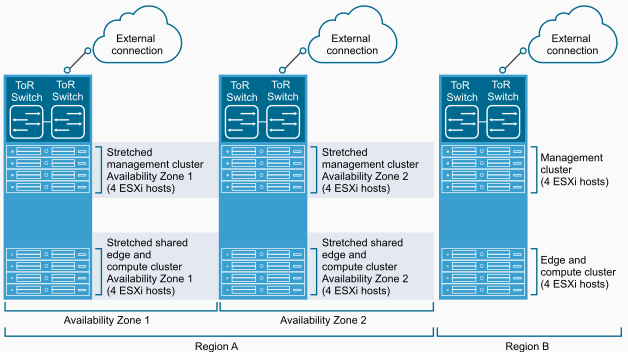
\includegraphics[width=0.95\textwidth]{imaxes/conceptosPrevios/zonasDispRegiones.png}
%   \caption{Una región contiene al menos una zona de disponibilidad.}
%   \label{fig:AVRegiones}
% \end{figure}
% \fi
%%%%%%%%%%%%%%%%%%%%%%%%%%%%%%%%%%%%%%%%%%%%%
%%%%%%%%%%%%%%%%%%%%%%%%%%%%%%%%%%%%%%%%%%%%%
%%%%%%%%%%%%%%%%%%%%%%%%%%%%%%%%%%%%%%%%%%%%%


